\chapter{Scripting 1}
\label{ch:scripting-1}

\begin{summary}
This chapter goes deeper into what constitutes a transaction and how scripting is used to lock bitcoins and later unlock them to spend them. Several examples are provided on how to create transactions by calling a node’s API or programmatically.
\end{summary}

\section{Transactions}

A transaction sends bitcoins from one address to another and it consists of 1+ inputs and 1+ outputs. The inputs of a transaction consist of outputs of previous transactions. When an output is spend it can never be used again\footnote{Think of cash. If you give a 20 euro note you can never reuse it. You might be given change but it will be different notes or coins.}. All the bitcoins are transferred elsewhere (to a recipient, back to yourself as change, etc.). Outputs that are available to be spend are called \emph{Unspent Transaction Outputs (UTXOs)} and Bitcoin nodes keep track of the complete UTXO set.

\begin{note}
Each time funds are sent to an address a new output (UTXO) is created. Thus, the balance of an address depends on all the UTXOs that correspond to it. Bitcoin wallets hide UTXOs to make the whole experience friendlier but some wallets allow you to specify which UTXOs you want to spend if needed. When we create transactions programmatically we will deal primarily with UTXOs.
\end{note}

When an output (UTXO) is created we also specify the conditions under which this output can be spend. When you specify an input (the UTXO of a previous transaction) to spend from you have to prove that you satisfy the conditions set by the UTXO.

The spending conditions and the proof that authorizes transfer are not fixed. A scripting language is used to define them. When a new output is created a script is placed in the UTXO called \keyword{scriptPubKey} or more informally locking script.

When we want to spend that UTXO we create a new transaction with an input that references the UTXO that we wish to spend together with an unlocking script or more formally a \keyword{scriptSig}.

The standard transaction output types supported by the Bitcoin protocol are:

\begin{itemize}
\item P2PK (Pay to Public Key - not used anymore)
\item P2MS (legacy multisignature transactions; now P2SH/P2WSH/P2TR are used instead)
\item P2PKH (Pay to Public Key Hash)
\item P2SH (Pay to Script Hash)
\item P2WPKH (Pay to Witness Public Key Hash)
\item P2WSH (Pay to Witness Script Hash)
\item P2TR (Pay to Taproot)
\item OP\_RETURN (allows for storing up to 80 bytes in an output)
\item Non-standard\footnote{Valid non-standard transactions (containing scripts other than those defined by the standard transaction output type scripts) are rejected and not relayed by nodes. However, they can be mined if it is arranged with a miner.} (any other valid transaction)
\end{itemize}

The most common transaction output type offering a standard way of transferring bitcoins around is P2PKH (and P2WPKH), which is effectively ``pay to a Bitcoin address''. It is also possible, and used in the past, to pay directly to a public key with P2PK but that is not used anymore. Another very important transaction output type is P2SH (and P2WSH) which allows locking scripts of arbitrary complexity to be used.

To define a locking and unlocking script we make use of a scripting language, simply called \emph{Script}\footnote{https://en.bitcoin.it/wiki/Script}. This relatively simple language consists of several operations each of them identified by an \emph{opcode} in hexadecimal. It is a simple stack-based language that uses reverse polish notation (e.g. \keyword{2 3 +}) and does not contain potentially dangerous programming constructs, like loops; it is a domain-specific language.

\subsection*{P2PKH}

Let’s examine the standard transaction of spending a Pay to Public Key Hash. The locking script (\keyword{scriptPubKey}) that secures the funds in a P2PKH address is the following:

\begin{emphbox}
\begin{verbatim}
OP_DUP OP_HASH160 <PKHash> OP_EQUALVERIFY OP_CHECKSIG
\end{verbatim}
\end{emphbox}

As we have seen in section \ref{sec:addresses} the public key hash (PKHash) can be derived from the Bitcoin address and vice versa. Thus, the above script locks the funds that have been sent in the address that corresponds to that PKHash.

To spend the funds the owner of the private key that corresponds to that address/PKHash needs to provide an unlocking script that if we prepend to the locking script the whole script will evaluate to true. An unlocking script for a P2PKH will look like this:

\begin{emphbox}
\begin{verbatim}
<Signature> <PublicKey>
\end{verbatim}
\end{emphbox}

Using the private key we provide an ECDSA signature of part of the transaction that we create (see section~\ref{sec:signatures} for more details). We also provide the public key\footnote{As we have already discussed in section~\ref{sec:addresses} the public key only appears in the blockchain after we spend from an address. This is where it appears!} for additional verification.

The validation to spend a UTXO consists of running the script of \keyword{scriptSig} plus \keyword{scriptPubKey}. Both scripts are added in the stack and executed as one script.

\subsection*{Validation of P2PKH Spending}
The validation process is described below in a step by step explanation during script execution. In each step, the script element evaluated will be highlighted (left column) and the current stack (right column) will also be displayed.

%\begin{table}
\begin{center}
\begin{longtable}[H]{ |L{0.47\linewidth}|L{0.47\linewidth}| }
\hline
\multicolumn{2}{|l|}{\emph{Step 0: Execution starts. Stack is empty.}}\\
\hline
\textsf{<Signature> <PublicKey> OP\_DUP OP\_HASH160 <PKHash> OP\_EQUALVERIFY OP\_CHECKSIG} & \\
\hline
\hline
\multicolumn{2}{|l|}{\emph{Step 1: First element is evaluated. It consists of data so it goes into the stack.}} \\
\hline
\textsf{{\color{blue}<Signature>} <PublicKey> OP\_DUP OP\_HASH160 <PKHash> OP\_EQUALVERIFY OP\_CHECKSIG} & \textsf{<Signature>} \\
\hline
\hline
\multicolumn{2}{|l|}{\emph{Step 2: Second element is also data and goes into the stack.}} \\
\hline
\textsf{<Signature> {\color{blue}<PublicKey>} OP\_DUP OP\_HASH160 <PKHash> OP\_EQUALVERIFY OP\_CHECKSIG} & \textsf{<Signature> <PublicKey>} \\
\hline
\hline
\multicolumn{2}{|l|}{\emph{Step 3: Next element is an operator that duplicates the top element of the stack.}}\\
\hline
\textsf{<Signature> <PublicKey> {\color{blue}OP\_DUP} OP\_HASH160 <PKHash> OP\_EQUALVERIFY OP\_CHECKSIG} & \textsf{<Signature> <PublicKey> <PublicKey>} \\
\hline
\hline
\multicolumn{2}{|L{0.94\linewidth}|}{\emph{Step 4: Next element is an operator that calcuates the HASH160 of the top stack element. HASH160 is equivalent to RIPEMD160( SHA256( element ) ) which is what is needed to calculate the PKH from a public key.}}\\
\hline
\textsf{<Signature> <PublicKey> OP\_DUP {\color{blue}OP\_HASH160} <PKHash> OP\_EQUALVERIFY OP\_CHECKSIG} & \textsf{<Signature> <PublicKey> <PKHash>} \\
\hline
\hline
\multicolumn{2}{|L{0.94\linewidth}|}{\emph{Step 5: Next element is data and it is pushed into the stack.}}\\
\hline
\textsf{<Signature> <PublicKey> OP\_DUP OP\_HASH160 {\color{blue}<PKHash>} OP\_EQUALVERIFY OP\_CHECKSIG} & \textsf{<Signature> <PublicKey> <PKHash> <PKHash>} \\
\hline
\hline
\multicolumn{2}{|L{0.94\linewidth}|}{\emph{Step 6: Next element is an operator that checks if the top two elements of the stack are equal and fails the script if they are not. Effectively this validates that the public key provided is indeed the one that corresponds to the PKH (or address) that we are trying to spend.}}\\
\hline
\textsf{<Signature> <PublicKey> OP\_DUP OP\_HASH160 <PKHash> {\color{blue}OP\_EQUALVERIFY} OP\_CHECKSIG} & \textsf{<Signature> <PublicKey>} \\
\hline
\hline
\multicolumn{2}{|L{0.94\linewidth}|}{\emph{Step 7: Next element is an operator that expects two elements from the stack; a signature and a public key that corresponds to that signature. If the signature is valid it returns true, otherwise false.}}\\
\hline
\textsf{<Signature> <PublicKey> OP\_DUP OP\_HASH160 <PKHash> OP\_EQUALVERIFY {\color{blue}OP\_CHECKSIG}} & \textsf{OP\_TRUE} \\
\hline
\end{longtable}
%\caption{Validation steps of P2PKH}
%\label{tab:p2pkh-validation}
\end{center}
%\end{table}

Since the script finished and the only element in the stack is now \keyword{OP\_TRUE}\footnote{Or OP\_1, i.e. true. All the operators, or opcodes, and their explanations can be found at https://en.bitcoin.it/wiki/Script} the node validated ownership of the UTXO and it is allowed to be spent. Success!

To help clarify how addresses, locking scripts and UTXOs relate please see figure~\ref{fig:utxos-pkhashes-addresses}. Addresses 1Zed, 1Alice and 1Bob are short for the actual bitcoin addresses of Zed, Alice and Bob respectively. The diagram emphasises what happens when funds are sent to an address.
\vspace{1em}

\begin{figure}[H]
\begin{center}
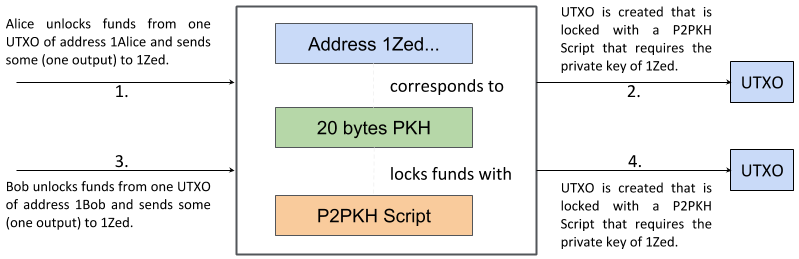
\includegraphics[scale=0.5]{images/utxos-pkhashes-addresses}
\caption{UTXOs, PKHashes and Addresses relationships.}
\label{fig:utxos-pkhashes-addresses}
\end{center}
\end{figure}

This section explained how funds residing in UTXOs are locked/unlocked and how scripts are evaluated for validation. In the next section we will go through several examples of how we can create simple transactions programmatically.



\section{Creating P2PKH Transactions}

In the previous section we went through transactions, their inputs and outputs and how the funds are locked. In this post we will go through different ways of creating a simple payment transaction from the command line and then programmatically. 

\subsection*{Automatically Create a Transaction}

We can use Bitcoin's build-in command \keyword{sendtoaddress} to send bitcoins to an address.

\begin{emphbox}
\begin{lstlisting}[style=Bash]
$ ./bitcoin-cli sendtoaddress mnB6gSoVfUAPu6MhKkAfgsjPfBWmEEmFr3 0.1
18f23a2c3bea97d30e0e09376222b6888943e7dc86df43ff5dfa1ff59c10d8ec
\end{lstlisting}
\end{emphbox}

In this example we use the node to send \keyword{0.1} bitcoins to a testnet address. Notice that we do not specify any details on which UTXOs to spend from. The node wallet will decide which UTXOs it will spend and in which address the change (there is almost always change) will go; i.e. we do not have any control when sending funds this way.

\begin{note}
Notice that the result is the transaction identifier (txid) of this transaction.
\end{note}


\subsection*{Creating a Transaction using a Node}

In this example we want to select the inputs explicitly. We need to know the txids and the output indexes (vout). As an example, we can get those with:

\begin{emphbox}
\begin{lstlisting}[style=Bash]
$ ./bitcoin-cli listunspent 0
[
  {
    "txid": "b3b7464d3472a9e83da4d5c179620b71724a62eac8bc14ac4543190227183940",
    "vout": 0,
    "address": "n1jnMQCyt9DHR3BYKzdbmXWM8M5UvH9nMW",
    "account": "",
    "scriptPubKey": "76a914ddcf9faf5625d6a96790710bbcef98af9a8719e388ac",
    "amount": 1.30000000,
    "confirmations": 0,
    "spendable": true,
    "solvable": true
  }
  ...
]
\end{lstlisting}
\end{emphbox}

The above command lists all UTXOs (even those with 0 confirmations; i.e. in the mempool). Now we can create a transaction specifying the UTXO that we want to spend.


\begin{emphbox}
\begin{lstlisting}[style=Bash]
$ ./bitcoin-cli createrawtransaction '''
> [
>  {
>   "txid": "b3b7464d3472a9e83da4d5c179620b71724a62eac8bc14ac4543190227183940",
>   "vout": 0
>  }
> ]
> ''' '''
> {
>  "mqazutWCSnuYqEpLBznke2ooGimyCtwCh8": 0.2
> }'''
0100000001403918...efbe09488ac00000000
\end{lstlisting}
\end{emphbox}


The result is the serialized raw transaction in hexadecimal. Note that this is not signed yet. To see the details of the raw transaction we can use:

\begin{emphbox}
\begin{lstlisting}[style=Bash]
$ ./bitcoin-cli decoderawtransaction 0100000001403918...efbe09488ac00000000
{
  "txid": "a7b54334096108e8f69ecfa19263cfbf2f12210165ef5fc2e98ef8e4e466392e",
  "hash": "a7b54334096108e8f69ecfa19263cfbf2f12210165ef5fc2e98ef8e4e466392e",
  "size": 85,
  "vsize": 85,
  "version": 1,
  "locktime": 0,
  "vin": [
   {
    "txid": "b3b7464d3472a9e83da4d5c179620b71724a62eac8bc14ac4543190227183940",
    "vout": 0,
    "scriptSig": {
      "asm": "",
      "hex": ""
    },
    "sequence": 4294967295
   }
  ],
  "vout": [
   {
    "value": 0.20000000,
    "n": 0,
    "scriptPubKey": {
      "asm": "OP_DUP OP_HASH160 6e751b60fcb566418c6b9f68bfa51438aefbe094\\
              OP_EQUALVERIFY OP_CHECKSIG",
      "hex": "76a9146e751b60fcb566418c6b9f68bfa51438aefbe09488ac",
      "reqSigs": 1,
      "type": "pubkeyhash",
      "addresses": [
        "mqazutWCSnuYqEpLBznke2ooGimyCtwCh8"
      ]
    }
   }
  ]
}
\end{lstlisting}
\end{emphbox}

We can confirm that this is unsigned because the unlocking script or \keyword{scriptSig} is empty. We now need to sign this transaction before it becames a valid transaction.

\begin{emphbox}
\begin{lstlisting}[style=Bash]
$ ./bitcoin-cli signrawtransactionwithwallet 01000000014039...be09488ac00000000
{
  "hex": "0100000001403918270...38aefbe09488ac00000000",
  "complete": true
}
\end{lstlisting}
\end{emphbox}

Now we have the final signed raw transaction (in attribute \keyword{hex}). If we use \keyword{decoderawtransaction} now you will see the unlocking script is properly set. We can test if this is a valid transaction before sending it to the node for broadcasting with the \keyword{mempoolaccept} command. Finally, we need to send it to the node for broadcasting.

\begin{emphbox}
\begin{lstlisting}[style=Bash]
$ ./bitcoin-cli sendrawtransaction 0100000001403918270...38aefbe09488ac00000000
error code: -26, error message:, 256: absurdly-high-fee
\end{lstlisting}
\end{emphbox}

In this instance we get an error saying that the transaction has an exceptionally high fee. We have not specified any output for change so \keyword{1.1} bitcoins would be given to miners (\keyword{1.3-0.2}). Most wallets have similar protection mechanisms to help safeguard from user errors.


\subsection*{Using HTTP JSON-RPC}

JSON-RPC is a simple protocol that specifies how to communicate with remote procedure calls using JSON as the format. It can be used with several transport protocols but most typically it is used over HTTP.

A user name and password has to be provided in \keyword{bitcoin.conf}. By default only local connections are allowed, but other connections can be allowed for trusted IPs with the \keyword{rpcallowip} configuration option.

\begin{emphbox}
rpcuser=kostas

rpcpassword=too\_long\_to\_guess
\end{emphbox}

Then we could use a tool like \keyword{curl} to make the JSON-RPC request:

\begin{emphbox}
\begin{lstlisting}[style=Bash]
$ curl --user kostas --data-binary '{"jsonrpc": "1.0", "id":"curltest",  \\
"method": "getblockcount", "params": [] }' -H 'content-type: text/plain;'\\
 http://127.0.0.1:18332/
Enter host password for user 'kostas':

{
  "result": 1746817,
  "error": null,
  "id": "curltest"
}
\end{lstlisting}
\end{emphbox}

Thus, we can also send the commands seen before to construct transactions via JSON-RPC.


\subsection*{Calling Node Commands Programmatically}
\label{ssec:calling-node-programmatically}

Library \keyword{python-bitcoin-utils}\footnote{The library can be installed directly with \keyword{pip install bitcoin-utils} in your working Python environment} wraps a Bitcon RPC library\footnote{https://github.com/jgarzik/python-bitcoinrpc} and provides a proxy object that allows a Python program to call all the CLI commands programmatically via JSON-RPC. For example:

\vspace{1em}
\begin{lstlisting}[style=Python]
from bitcoinutils.setup import setup
from bitcoinutils.proxy import NodeProxy

# always remember to setup the network
setup('testnet')

# get a node proxy using default host and port
proxy = NodeProxy('rpcuser', 'rpcpw').get_proxy()

# call the node's getblockcount JSON-RPC method
count = proxy.getblockcount()

print(count)
\end{lstlisting}
\vspace{1em}

All API calls can be used, including the ones to create a transaction with either \keyword{sendtoaddress} or \keyword{createrawtransaction} + \keyword{signrawtransaction} + \keyword{sendrawtransaction}.



\subsection*{Creating Transactions Programmatically}

The Bitcoin node allows the creation of basic transactions but it does not support arbitrary scripts. We can create those programmatically by explicitly specifying the locking/unlocking conditions. We will use the \keyword{python-bitcoin-utils} library to demonstrate.

There are several examples included in the library that you can consult, like the most common transaction, a P2PKH payment\footnote{\url{https://github.com/karask/python-bitcoin-utils/blob/b31c82e7005e06db7f780688cfcd9332d479f39d/examples/p2pkh_transaction.py}} with one input and two outputs (the second output being the change).

\vspace{1em}
\begin{lstlisting}[style=Python]
# Copyright (C) 2018-2020 The python-bitcoin-utils developers
#
# This file is part of python-bitcoin-utils
#
# It is subject to the license terms in the LICENSE file found in the top-level
# directory of this distribution.
#
# No part of python-bitcoin-utils, including this file, may be copied,
# modified, propagated, or distributed except according to the terms contained
# in the LICENSE file.

from bitcoinutils.setup import setup
from bitcoinutils.utils import to_satoshis
from bitcoinutils.transactions import Transaction, TxInput, TxOutput
from bitcoinutils.keys import P2pkhAddress, PrivateKey
from bitcoinutils.script import Script

def main():
    # always remember to setup the network
    setup('testnet')

    # create transaction input from tx id of UTXO (contained 0.4 tBTC)
    txin = TxInput('fb48f4e23bf6ddf606714141ac78c3e921c8c0bebeb7c8abb2c799e9ff96ce6c', 0)

    # create transaction output using P2PKH scriptPubKey (locking script)
    addr = P2pkhAddress('n4bkvTyU1dVdzsrhWBqBw8fEMbHjJvtmJR')
    txout = TxOutput(to_satoshis(0.1), Script(['OP_DUP', 'OP_HASH160', addr.to_hash160(),
                                  'OP_EQUALVERIFY', 'OP_CHECKSIG']) )

    # create another output to get the change - remaining 0.01 is tx fees
    # note that this time we used to_script_pub_key() to create the P2PKH
    # script
    change_addr = P2pkhAddress('mmYNBho9BWQB2dSniP1NJvnPoj5EVWw89w')
    change_txout = TxOutput(to_satoshis(0.29), change_addr.to_script_pub_key())
    #change_txout = TxOutput(to_satoshis(0.29), Script(['OP_DUP', 'OP_HASH160',
    #                                     change_addr.to_hash160(),
    #                                     'OP_EQUALVERIFY', 'OP_CHECKSIG']))

    # create transaction from inputs/outputs -- default locktime is used
    tx = Transaction([txin], [txout, change_txout])

    # print raw transaction
    print("\nRaw unsigned transaction:\n" + tx.serialize())

    # use the private key corresponding to the address that contains the
    # UTXO we are trying to spend to sign the input
    sk = PrivateKey('cRvyLwCPLU88jsyj94L7iJjQX5C2f8koG4G2gevN4BeSGcEvfKe9')

    # note that we pass the scriptPubkey as one of the inputs of sign_input
    # because it is used to replace the scriptSig of the UTXO we are trying to
    # spend when creating the transaction digest
    from_addr = P2pkhAddress('myPAE9HwPeKHh8FjKwBNBaHnemApo3dw6e')
    sig = sk.sign_input( tx, 0, Script(['OP_DUP', 'OP_HASH160',
                                       from_addr.to_hash160(), 'OP_EQUALVERIFY',
                                       'OP_CHECKSIG']) )

    # get public key as hex
    pk = sk.get_public_key().to_hex()

    # set the scriptSig (unlocking script)
    txin.script_sig = Script([sig, pk])
    signed_tx = tx.serialize()

    # print raw signed transaction ready to be broadcasted
    print("\nRaw signed transaction:\n" + signed_tx)


if __name__ == "__main__":
    main()
\end{lstlisting}
\vspace{1em}

This produces the serialized raw transaction in hexadecimal. We can then use \keyword{sendrawtransaction} to broadcast this to the Bitcoin network. Notice that the transaction identifier used to create the input is hardcoded for simplicity; in an actual program we would call \keyword{listunspent} to find the available UTXOs.



\section{Signatures}
\label{sec:signatures}

In this section we will explain how and what needs to be signed to prove ownership of funds residing in specific addresses. 

When we create a new transaction we need to provide a signature for each UTXO that we want to spent. For a P2PKH UTXO the signature proves:

\begin{itemize}
\item that the signer is the owner of the private key
\item the proof of authorization is undeniable
\item the parts of the tx that were signed cannot be modified after it has been signed
\end{itemize}

The digital signature algorithm used is ECDSA and each signature is serialized using DER. There are different ways to sign inputs of a transaction so as to provide different commitments. For example: ``I agree to spend this input and sign it as long as no one can change the outputs I specified''. To specify these commitments, i.e. which parts of the transaction will be signed, we add a special 1 byte flag called SIGHASH at the end of the DER signature.

Each transaction input needs to be signed separately from others. Parts of the new transaction will be hashed to create a digest and the digest is what is signed and included in the unlocking script. To determine which parts are hashed the following rules are followed:

\begin{itemize}
\item all other inputs’ unlocking scripts (scriptSigs) should be empty
\item the input’s unlocking script (scriptSig), the one that we sign, should be set to the locking script (scriptPubKey) of the UTXO that we are trying to spend
\item follow additional rules according to the SIGHASH flag
\end{itemize}

The possible SIGHASH flags, values and meaning are:

\begin{description}
\item[\keyword{ALL (0x01)}] Signs all the inputs and outputs, protecting everything except the signature scripts against modification. This transaction is final and no one can modify it without invalidating this signature.
\item[\keyword{NONE (0x02)}] Signs all of the inputs but none of the outputs, allowing anyone to change where the satoshis are going. A miner will always be able to send the funds to his address.
%This flag is useful in combination with another inputs’ signatures using, say, \keyword{ALL} to secure the outputs. 
	It can also be used to send funds somewhere as long as everybody else also sends funds; in this case it is assumed that one of the signers will use SIGHASH \keyword{ALL} (or \keyword{SINGLE}) to lock the outputs before broadcasting. It can be used as a blank check to a miner. 
\item[\keyword{SINGLE (0x03)}] Sign all the inputs and only one output, the one corresponding to this input (the output with the same output index number as this input), ensuring nobody can change your part of the transaction but allowing other signers to change their part of the transaction. The corresponding output must exist. It can be used if someone creates a transaction with some inputs that they cannot spend and specific outputs and then send to other participants, one of which will to sign (with \keyword{ALL} or \keyword{SINGLE}), if they agree. A concrete example is provided later in this section.
\item[\keyword{ALL|ANYONECANPAY (0x81)}] Signs only this one input and all the outputs. It allows anyone to add or remove inputs, so anyone can contribute additional satoshis but they cannot change how many satoshis are sent not where they go. It can be used to implement kickstarter-style crowdfunding.
\item[\keyword{NONE|ANYONECANPAY (0x82)}] Signs only this one input and allows anyone to add or remove other inputs or outputs, so anyone who gets a copy of this input can spend it however they like. This input can be spend even in another transaction!
\item[\keyword{SINGLE|ANYONECANPAY (0x83)}] Signs this one input and its corresponding output. Allows anyone to add or remove other inputs. A potential use would be as a means to exchange colored coin\footnote{https://en.bitcoin.it/wiki/Colored\_Coins} tokens with satoshis. For example, one can create a transaction that has an input which holds 10 of their tokens and an output of 10 million satoshis to an address that they own. This transaction would be invalid since the inputs do not provide the 10 million satoshis but it can be shared with others. If someone wants to claim the 10 tokens they can add an input with at least 10 million satoshis and an output that sends the 10 tokens to them. This would complete the transaction which can then be broadcasted.
\end{description}

\begin{figure}[H]
\begin{center}
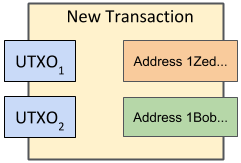
\includegraphics[scale=0.5]{images/example-transaction}
\caption{Example transaction with two inputs and two outputs.}
\label{fig:example-transaction}
\end{center}
\end{figure}

For an example of \keyword{SINGLE}, consider creating the transaction shown above. Alice needs to pay 1.5 bitcoins to Zed and they agreed with Bob that he will contribute 0.5 of that amount. Then Alice creates a transaction with two inputs, UTXO1 that she owns (with 1 BTC) and UTXO2 that Bob owns (with 1 BTC) and a single output that sends 1.5 bitcoins to Zed. She signed UTXO1 with SIGHASH \keyword{SINGLE} and sends the incomplete transaction to Bob. Bob cannot choose a UTXO other than UTXO2 since it will invalidate Alice’s signature of UTXO1. However, he is free to add other outputs so he creates an output that sends the remaining bitcoins (he agreed to pay only 0.5) to one of his addresses. He can then sign UTXO2 with SIGHASH \keyword{ALL} which will effectively finalize the transaction\footnote{No more input or output changes are allowed without invalidating this signature.}. Note that:

\begin{itemize}
\item The sequence numbers of other inputs are not included in the signature, and can be updated.
\item As already demonstrated above, with multiple inputs, each signature hash type can sign different parts of the transaction. If a 2-input transaction has one input signed with \keyword{NONE} and the other with \keyword{ALL}, the \keyword{ALL} signer can choose where to spend the funds without consulting the \keyword{NONE} signer.
\end{itemize}


\section{Pay to script hash (P2SH)}
\label{sec:p2sh}

This section explains the rationale behind Pay to Script Hash (P2SH) type of addresses and demonstrates with code.

\subsection*{Multi-signature transaction output type}
To demonstrate the advantages of P2SH we will first go through a simple use case using first P2MS, the legacy multisignature standard transaction output type, and then implement the same script with the P2SH standard transaction output type.

Consider the scenario where we accept funds in an address that is not controlled by one person. For example it is typical for companies to allow spending from corporate accounts only if, say, 2 people agree. These are called multi-signature accounts. A multi-signature account requires M-of-N signatures in order to spend the funds. An address’ locking script could enforce that. For example a 2-of-3 multi-signature locking script would look like:

\begin{emphbox}
\begin{lstlisting}[style=Pseudomath]
2 <Director's Public Key> <CFO's Public Key> <COO's Public Key> 
3 CHECKMULTISIG
\end{lstlisting}
\end{emphbox}

Indeed, this is the locking script of the multisignature standard transaction output type. If someone needs to send money (lock funds) to that output script then they need to know it! The company would need to send this script to all their customers that wish to pay them.

This is not practical since the whole script is recorded on the blockchain for every transaction and more importantly has privacy issues; the company is revealing the public keys that control the funds.

If you think about it the precise locking/unlocking script of the funds should not concern the customers at all. Only the company should know how to spend them.


\subsection*{Pay to script hash (P2SH)}
P2SH is a type of transaction output (BIP-16\footnote{https://github.com/bitcoin/bips/blob/master/bip-0016.mediawiki}) that moves the responsibility for supplying the conditions to redeem a transaction (locking script) from the sender of the funds to the redeemer (receiver).

The locking script of such a transaction is quite simple:

\begin{emphbox}
\begin{lstlisting}[style=Pseudomath]
OP_HASH160 [20-byte-hash-value] OP_EQUAL
\end{lstlisting}
\end{emphbox}

The 20-byte hash value is the hash of the redeem script:

\begin{emphbox}
\begin{lstlisting}[style=Pseudomath]
RIPEMD-160( SHA-256( 2 <Director's Public Key> <CFO's Public Key> 
<COO's Public Key> 3 CHECKMULTISIG ) )
\end{lstlisting}
\end{emphbox}

Using this hash we create a Bitcoin address (same process as described in section~\ref{ssec:legacy-addresses} but instead of \keyword{OP\_HASH160(pubkey)} we use \keyword{OP\_HASH160(redeem script)}) using the version prefix of \keyword{0x05} that creates addresses that start with \keyword{3}. 

We then only need to disseminate this address to the company’s customers. They can send funds oblivious to how these funds are locked. The company knows how they are unlocked so they can prepare the appropriate unlocking script.

As an example, to spend the funds, the company can create the following script:

\begin{emphbox}
\begin{lstlisting}[style=Pseudomath]
<Director's signature> <CFO's signature> 
<2 <Director's Public Key> <CFO's Public Key> <COO's Public Key> 
 3 CHECKMULTISIG>
\end{lstlisting}
\end{emphbox}

It has two parts, the redeem script’s unlocking conditions (which in this case are two of the signatures) plus the redeem script. Notice how the redeem script is revealed only when the company spends the funds; and it only reveals the two signatures, not all three.

Validation occurs in the following steps:

Initially, the scriptSig part is pushed into the stack and then the stack is copied for later use. The copy would look like:

\begin{emphbox}
\begin{lstlisting}[style=Pseudomath]
<Director's signature> <CFO's signature>
<2 <Director's Public Key> <CFO's Public Key> <COO's Public Key>
 3 CHECKMULTISIG>
\end{lstlisting}
\end{emphbox}

Then the execution continues normally:

\begin{emphbox}
\begin{lstlisting}[style=Pseudomath]
<Director's signature> <CFO's signature>
<2 <Director's Public Key> <CFO's Public Key> <COO's Public Key>
 3 CHECKMULTISIG>  OP_HASH160 [20-byte-hash-value] OP_EQUAL
\end{lstlisting}
\end{emphbox}

If the hashed redeem script is equal to the 20-byte hash value the above script will result \keyword{OP\_TRUE} in the top of the stack, which validates that the correct redeem script was passed. We can now proceed in validating the actual redeem script. We do this by using the copy of the stack, by first deserializing the top element (redeem script) and then executing normally:

\begin{emphbox}
\begin{lstlisting}[style=Pseudomath]
<Director's signature> <CFO's signature> 2
<Director's Public Key> <CFO's Public Key> <COO's Public Key>
3 CHECKMULTISIG
\end{lstlisting}
\end{emphbox}

If that also results to \keyword{OP\_TRUE} then the funds can be spend.

\subsection*{Summary / Advantages}
P2SH moves the responsibility for supplying the conditions to redeem a transaction (locking script) from the sender of the funds to the redeemer (receiver).

\begin{itemize}
\item P2SH allows us to create arbitrary redeem scripts; we can thus create quite complex scripts and not be limited to the few standard transaction output types.
\item Reduces the size of the funding transactions typically resulting in saving blockchain sace.
\item Increases privacy by hiding the locking conditions.
\end{itemize}

\subsection*{Example: create a P2SH address based on a P2PK script}
As we have seen P2SH allows us to wrap arbitrary scripts hiding the script itself until it is spend. To demonstrate we will wrap a simple P2PK script and display the P2SH address that corresponds to that script.

\vspace{1em}
\begin{lstlisting}[style=Python]
from bitcoinutils.setup import setup
from bitcoinutils.keys import P2shAddress, PrivateKey
from bitcoinutils.script import Script


def main():
    # always remember to setup the network
    setup('testnet')

    #
    # This script creates a P2SH address containing a P2PK locking script
    #

    # secret key corresponding to the pubkey needed for the P2PK locking
    p2pk_sk = PrivateKey('cRvyLwCPLU88jsyj94L7iJjQX5C2f8koG4G2gevN4BeSGcEvfKe9')

    # get the public key
    p2pk_pk = p2pk_sk.get_public_key()

    # get the address (from the public key)
    p2pk_addr = p2pk_pk.get_address()

    # create the redeem script
    redeem_script = Script([p2pk_pk.to_hex(), 'OP_CHECKSIG'])

    # create a P2SH address from a redeem script
    addr = P2shAddress.from_script(redeem_script)
    print(addr.to_string())

if __name__ == "__main__":
    main()
\end{lstlisting}
\vspace{1em}

The result is address \keyword{2MvzN3FntupGqY66FuGzoK9HFXqPFyMxfVU} which can be shared to anyone that wishes to send us some funds.


\subsection*{Example: spend funds from a P2SH address}
Assuming that someone has sent funds to the P2SH address we just created let us spend it programmatically. Again, we will hardcode the UTXOs for brevity but we can always use the proxy object mentioned in section~\ref{ssec:calling-node-programmatically} to get the UTXOs programmatically.

\vspace{1em}
\begin{lstlisting}[style=Python]
from bitcoinutils.setup import setup
from bitcoinutils.utils import to_satoshis
from bitcoinutils.transactions import Transaction, TxInput, TxOutput
from bitcoinutils.keys import P2pkhAddress, P2shAddress, PrivateKey
from bitcoinutils.script import Script

def main():
    # always remember to setup the network
    setup('testnet')

    #
    # This script spends from a P2SH address containing a P2PK script
    #

    # create transaction input from tx id of UTXO (contained 0.1 tBTC)
    txin = TxInput('7db363d5a7fabb64ccce154e906588f1936f34481223ea8c1f2c935b0a0c945b', 0)

    # secret key needed to spend P2PK that is wrapped by P2SH
    p2pk_sk = PrivateKey('cRvyLwCPLU88jsyj94L7iJjQX5C2f8koG4G2gevN4BeSGcEvfKe9')
    p2pk_pk = p2pk_sk.get_public_key().to_hex()
    # create the redeem script - needed to sign the transaction
    redeem_script = Script([p2pk_pk, 'OP_CHECKSIG'])

    to_addr = P2pkhAddress('n4bkvTyU1dVdzsrhWBqBw8fEMbHjJvtmJR')
    txout = TxOutput(to_satoshis(0.09), to_addr.to_script_pub_key() )

    # no change address - the remaining 0.01 tBTC will go to miners)

    # create transaction from inputs/outputs -- default locktime is used
    tx = Transaction([txin], [txout])

    # print raw transaction
    print("\nRaw unsigned transaction:\n" + tx.serialize())

    # use the private key corresponding to the address that contains the
    # UTXO we are trying to spend to create the signature for the txin -
    # note that the redeem script is passed to replace the scriptSig
    sig = p2pk_sk.sign_input(tx, 0, redeem_script )

    # set the scriptSig (unlocking script)
    txin.script_sig = Script([sig, redeem_script.to_hex()])
    signed_tx = tx.serialize()

    # print raw signed transaction ready to be broadcasted
    print("\nRaw signed transaction:\n" + signed_tx)
    print("\nTxId:", tx.get_txid())


if __name__ == "__main__":
    main()
\end{lstlisting}
\vspace{1em}

\begin{note}
As already mentioned, the first time we spend from the address, i.e. broadcasting this transaction, reveals the redeem script to everyone.
\end{note}



\section{Segregated Witness (SegWit)}
\label{sec:segwit}

In this section we will briefly explain what Segregated Witness is, what it changes and how we can create segwit scripts programmatically. 

Segregated Witness is a consensus change that introduces an update on how transactions are constructed. In particular it separates (segregates) the unlocking script (witness) from the rest of the input; a transaction input does not contain an unlocking script anymore and the latter is found in another structure that goes alongside the transaction. 

To illustrate see figure~\ref{fig:tx-with-without-segwit} (i) for the original transaction that we used as an example in chapter~\ref{ch:howbitcoinworks}. We can see that the unlocking script is part of the input that we are spending. In (ii) we can see the segwit equivalent transaction where the unlocking script (\keyword{scriptSig}) is empty and it is moved outside the transaction.

\begin{figure}[H]
\begin{center}
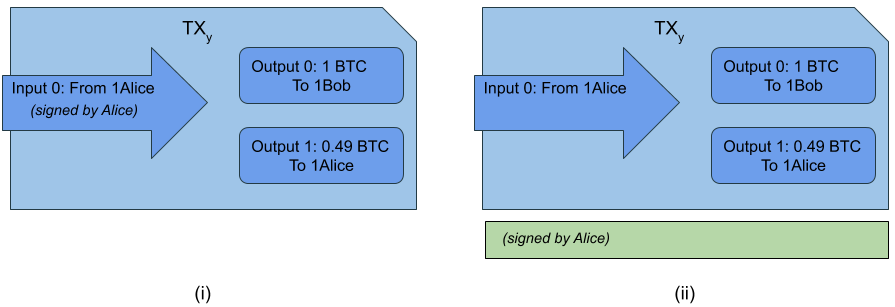
\includegraphics[scale=0.5]{images/tx-with-without-segwit}
\caption{Example transaction with (i) a non-segwit input and (ii) a segwit input.}
\label{fig:tx-with-without-segwit}
\end{center}
\end{figure}

The segwit upgrade is described in detail in BIPs\footnote{Bitcoin Improvement Proposals} 141, 143, 144 and 145 and it provides several benefits\footnote{https://bitcoincore.org/en/2016/01/26/segwit-benefits/}. We will examine two of them here: \emph{transaction malleability} and \emph{effective block size increase}.

\subsection*{Transaction malleability}
Each transaction is uniquely identified by its \emph{transaction identifier} or \keyword{txid}. The \keyword{txid} is constructed by hashing\footnote{The SHA-256 hashing algorithm is applied twice.} the serialized transaction (the blue part of figure~\ref{fig:tx-with-without-segwit}).

It is possible to slightly change the unlocking script, e.g. by a miner, so as the resulting transaction is semantically identical to the original; thus still valid. This can be accomplished, for example, by slightly changing the structure of the signature\footnote{DER allows for some flexibility on how to encode the signature.}.

That is a problem because given how the \keyword{txid} is created even the slightest modification will change the \keyword{txid}. While the transaction is identical, i.e. funds will be moved exactly as intended, our ability to monitor this transaction is problematic given that we will be checking for confirmations in a \keyword{txid} that is not valid anymore.

With segwit inputs, however, the unlocking script (the green part of figure~\ref{fig:tx-with-without-segwit} (ii) ) is not part of the \keyword{txid} construction and thus it is impossible to modify it. A non-malleable \keyword{txid} is more reliable and allows for more advanced scripts/solutions like the lightning network.


\subsection*{Effective block size increase}
The actual block size remains the same, at 1MB. However, the unlocking scripts are now not counted as part of the block and thus more transactions can fit into the 1MB limit.

Segwit introduces the concept of block \emph{weight}, a new metric for the size of blocks. A block can have a maximum weight of 4MBs. The non-witness part bytes of a transaction are now multiplied by 4 to get its weight while the witness part bytes are multiplied by 1, a discount of 75\%. This allows for an effective block size increase of about 2.8x, if all transactions use segwit\footnote{E.g. block 748918 reached 2.77 MBs because it included a lot of P2WSH 2-of-3 multi-signature scripts.}.

The \emph{virtual} size, or \keyword{vsize} of a transaction is the size in bytes of a transaction including the segwit discount. For non-segwit transactions\footnote{I.e. transaction with no segwit inputs.} \keyword{size} and \keyword{vsize} are identical.


\subsection*{Segwit transaction output types}
Segwit introduces two new transaction types, \emph{Pay-to-Witness-Public-Key-Hash (P2WPKH)} and \emph{Pay-to-Witness-Script-Hash (P2WSH)}, which are the segwit equivalent of P2PKH and P2SH respectively. They are sometimes called \emph{native} segwit to differentiate from \emph{nested} segwit.

The locking script (\keyword{scriptPubKey}) of these new types consists of two elements, a \keyword{version byte} and the \keyword{witness program}. The version byte introduces versioning in the witness program of the script. That is another benefit of segwit, since it allows for easy updates based on a new version.

Remember, that when signing to spend any output we need to provide the locking script, which is used to substitute the \keyword{scriptPubKey} before we calculate the transaction digest and sign it. For segwit transaction types each witness program corresponds to a predefined template script that is called \keyword{scriptCode}.

For example the \keyword{scriptCode} for a P2WPKH output is:

\begin{emphbox}
\begin{lstlisting}[style=Pseudomath]
OP_DUP OP_HASH160 <pubkey-hash> OP_EQUALVERIFY OP_CHECKSIG
\end{lstlisting}
\end{emphbox}

where the pubkey-hash is substituted with the witness program. Note that this is used for calculating the digest and not for validation (see next section).

\subsubsection*{P2WPKH}
In segwit version 0, a P2WPKH witness program is just the 20-byte public key hash. The unlocking script (\keyword{scriptSig}) should be empty and the witness structure contains the unlocking script.

\begin{emphbox}
\begin{lstlisting}[style=Pseudomath]
scriptPubKey: 0 6b85f9a17492c691c1d861cc1c722ff683b27f5a
scriptSig:
witness: <signature> <pubkey>
\end{lstlisting}
\end{emphbox}

The validation is executed as follows:
\begin{enumerate}
\item The `0' in scriptPubKey specifies that the following is a version 0 witness program.
\item The length of the witness program (20-bytes) indicates that it is a P2WPKH type.
\item The witness must consist of exactly two items.
\item The \keyword{HASH160} of the <pubkey> must match the 20-bytes witness program.
\item Finally, the signature is verified by: \keyword{<signature> <pubkey> CHECKSIG}.
\end{enumerate}

The \keyword{scriptCode} for P2WPKH is identical to P2PKH.


\subsubsection*{P2WSH}
In segwit version 0, a P2WSH witness program is just the 32-byte script hash. The unlocking script (\keyword{scriptSig}) should be empty and the witness structure\footnote{The witness structure contains all the witnesses, or \emph{script witnesses} depending on how many inputs are Segwit. Witnesses are the equivalent of the scriptSig in P2SH outputs.} contains the unlocking script as well as the \emph{witness script}\footnote{To clarify, witness script for a P2WSH is exactly what redeem script is for a P2SH.}.

\begin{emphbox}
\begin{lstlisting}[style=Pseudomath]
scriptPubKey: 0 3b892c61cc15f9a17<32 bytes>c1c722ff683b27f5a
scriptSig:
witness: 0 <signature1> <1 <pubkey1> <pubkey2> 2 CHECKMULTISIG>
\end{lstlisting}
\end{emphbox}

The validation is executed as follows:
\begin{enumerate}
\item The `0' in scriptPubKey specifies that the following is a version 0 witness program.
\item The length of the witness program (32-bytes) indicates that it is a P2WSH type.
\item The witness must consist of the unlocking script followed by the witness script) 
\item The \keyword{SHA256} of the witness script must match the 32-bytes witness program
\item Finally, the witness script is deserialized and executed after the remaining witness stack: \keyword{0 <signature1> \emph{1 <pubkey1> <pubkey2> 2 CHECKMULTISIG}}.
\end{enumerate}

The \keyword{scriptCode} for P2WSH is the witness script.


\subsection*{Nested Segwit transaction output types}
It is possible for a non-segwit aware wallet to pay to a segwit address by embedding P2WPKH or P2WSH into a P2SH. The recipient will provide a P2SH address to the sender who can send funds as usual. The recipient can then use the redeem script which is actually the witness script to spend the funds.

\subsubsection*{P2SH(P2WPKH)}
Get the hash of the P2WPKH \keyword{scriptPubKey} and use it in P2SH as usual:

\begin{emphbox}
\begin{lstlisting}[style=Pseudomath]
HASH160 (0 6b85f9a17492c691c1d861cc1c722ff683b27f5a)
\end{lstlisting}
\end{emphbox}

And thus:

\begin{emphbox}
\begin{lstlisting}[style=Pseudomath]
scriptPubKey: <HASH160 <20-byte-script-hash> EQUAL
scriptSig: <0 <20-byte-key-hash>>
witness: <signature> <pubkey>
\end{lstlisting}
\end{emphbox}

Note that for spending\footnote{From a segwit-aware wallet.} the \keyword{scriptSig} contains the redeem script as a single element and without any extra unlocking data before it since those are in witness (check section~\ref{sec:p2sh} for how P2SH works). 

For validation the \keyword{scriptSig} is hashed with \keyword{HASH160} and compared to the \keyword{<20-byte-script-hash>} in \keyword{scriptPubKey}. If they are equal we can then verify the public key and signature as a native P2WPKH.


\subsubsection*{P2SH(P2WSH)}
Get the hash of the P2WSH \keyword{scriptPubKey} and use it in P2SH as usual:

\begin{emphbox}
\begin{lstlisting}[style=Pseudomath]
HASH160 (0 3b892c61cc15f9a17<32 bytes>c1c722ff683b27f5a)
\end{lstlisting}
\end{emphbox}

And thus:

\begin{emphbox}
\begin{lstlisting}[style=Pseudomath]
scriptPubKey: <HASH160 <20-byte-script-hash> EQUAL
scriptSig: <0 <32-byte-witness-script-hash>>
witness: 0 <signature1> <1 <pubkey1> <pubkey2> 2 CHECKMULTISIG>
\end{lstlisting}
\end{emphbox}

Note that for spending the \keyword{scriptSig} contains the witness script as a single element and without any extra unlocking data before it since those are in witness (check section~\ref{sec:p2sh} for how P2SH works).

For validation the \keyword{scriptSig} is hashed with \keyword{HASH160} and compared to the \keyword{<20-byte-script-hash>} in \keyword{scriptPubKey}. If they are equal we can then verify the witness script as a native P2WSH.


\subsection*{Implemented as a soft-fork}
Changing the transaction format is normally a hard-fork. The new transactions would not be accepted by the nodes running the old software. To go around that and implement the new functionality as a soft-fork additional effort was required. Without going into too much details:


\begin{itemize}
\item The original transaction format was not changed. The \keyword{scriptSig} would just be empty and the \keyword{witnesses} would go in a new structure.
\item The header \emph{should} represent the whole block and thus a witness merkle root is calculated (from all transactions' witness scripts) and included in an \keyword{OP\_RETURN} output (see section~\ref{sec:storing-data}) of the coinbase transaction. Being in the coinbase means that the witnesses are represented in the header via the \keyword{hashMerkleRoot} (see section~\ref{sec:mining-technical} for a reminder).
\item Witness data are provided only when nodes ask for them and thus old nodes will get blocks without the witness data, i.e. new nodes will remove witness data before relaying the blocks to old nodes. To old nodes, segwit blocks would look like blocks that contain some non-standard transactions.
\item Old nodes trying to spend a segwit output would violate the clean stack rule\footnote{If there are more than one elements after execution the stack is not \emph{clean} and is considered non standard for legacy transactions. For segwit v0 (P2WSH) and Tapscript they are considered invalid.}; OP\_0 <bytes in hex> will remain in the stack.
\end{itemize}


\subsection*{Example: spend a native segwit output type}
Assuming that a P2WPKH address have some funds (UTXOs) we can use the following code to send some funds to a legacy address. As usual, we hardcode the UTXOs for simplicity.

\vspace{1em}
\begin{lstlisting}[style=Python]
from bitcoinutils.setup import setup
from bitcoinutils.utils import to_satoshis
from bitcoinutils.transactions import Transaction, TxInput, TxOutput
from bitcoinutils.keys import P2pkhAddress, PrivateKey
from bitcoinutils.script import Script

def main():
    # always remember to setup the network
    setup('testnet')

    # the key that corresponds to the P2WPKH address
    priv = PrivateKey("cVdte9ei2xsVjmZSPtyucG43YZgNkmKTqhwiUA8M4Fc3LdPJxPmZ")

    pub = priv.get_public_key()

    fromAddress = pub.get_segwit_address()
    print(fromAddress.to_string())

    # amount is needed to sign the segwit input
    fromAddressAmount = to_satoshis(0.01)

    # UTXO of fromAddress
    txid = '13d2d30eca974e8fa5da11b9608fa36905a22215e8df895e767fc903889367ff'
    vout = 0

    toAddress = P2pkhAddress('mrrKUpJnAjvQntPgz2Z4kkyr1gbtHmQv28')

    # create transaction input from tx id of UTXO
    txin = TxInput(txid, vout)

    # script code required for signing; for p2wpkh it is the same as p2pkh
    script_code = Script(['OP_DUP', 'OP_HASH160', pub.to_hash160(),
                           'OP_EQUALVERIFY', 'OP_CHECKSIG'])

    # create transaction output
    txOut = TxOutput(to_satoshis(0.009), toAddress.to_script_pub_key())

    # create transaction without change output - if at least a single input is
    # segwit we need to set has_segwit=True
    tx = Transaction([txin], [txOut], has_segwit=True)

    print("\nRaw transaction:\n" + tx.serialize())

    sig = priv.sign_segwit_input(tx, 0, script_code, fromAddressAmount)
    tx.witnesses.append( Script([sig, pub.to_hex()]) )

    # print raw signed transaction ready to be broadcasted
    print("\nRaw signed transaction:\n" + tx.serialize())
    print("\nTxId:", tx.get_txid())


if __name__ == "__main__":
    main()
\end{lstlisting}
\vspace{1em}


\subsection*{Example: spend a nested segwit output type}
As described above we can also nest the new segwit address output types in a P2SH so that old non-segwit clients can send funds to new segwit-supporting clients. This example spends such a UTXO demonstrating a couple of additional details that need to be taken into consideration.

\vspace{1em}
\begin{lstlisting}[style=Python]
from bitcoinutils.setup import setup
from bitcoinutils.utils import to_satoshis
from bitcoinutils.keys import PrivateKey, P2pkhAddress, P2shAddress
from bitcoinutils.transactions import Transaction, TxInput, TxOutput
from bitcoinutils.script import Script

def main():
    # always remember to setup the network
    setup('testnet')

    # the key that corresponds to the P2WPKH address
    priv = PrivateKey('cNho8fw3bPfLKT4jPzpANTsxTsP8aTdVBD6cXksBEXt4KhBN7uVk')
    pub = priv.get_public_key()

    # the p2sh script and the corresponding address
    redeem_script = pub.get_segwit_address().to_script_pub_key()
    p2sh_addr = P2shAddress.from_script(redeem_script)

    # the UTXO of the P2SH-P2WPKH that we are trying to spend
    inp = TxInput('95c5cac558a8b47436a3306ba300c8d7af4cd1d1523d35da3874153c66d99b09', 0)

    # exact amount of UTXO we try to spent
    amount = 0.0014

    # the address to send funds to
    to_addr = P2pkhAddress('mvBGdiYC8jLumpJ142ghePYuY8kecQgeqS')

    # the output sending 0.001 -- 0.0004 goes to miners as fee -- no change
    out = TxOutput(to_satoshis(0.001), to_addr.to_script_pub_key())

    # create a tx with at least one segwit input
    tx = Transaction([inp], [out], has_segwit=True)

    # script code is the script that is evaluated for a witness program type; each
    # witness program type has a specific template for the script code;
    # the script code that corresponds to P2WPKH is the same as P2PKH
    script_code = pub.get_address().to_script_pub_key()

    # calculate signature using the appropriate script code
    # remember to include the original amount of the UTXO
    sig = priv.sign_segwit_input(tx, 0, script_code, to_satoshis(amount))

    # script_sig is the redeem script passed as a single element
    inp.script_sig = Script([redeem_script.to_hex()])

    # finally, the unlocking script is added as a witness
    tx.witnesses.append(Script([sig, pub.to_hex()]))

    # print raw signed transaction ready to be broadcasted
    print("\nRaw signed transaction:\n" + tx.serialize())

if __name__ == "__main__":
    main()
\end{lstlisting}
\vspace{1em}


\section{Pay To Multi-signature (P2MS)}
Pay to multi-signature or \emph{Pay-to-Multisig} is a standard output type that was introduced before P2SH. Its aim was to provide a way for bitcoins to be locked by several public keys which could belong to different people. Typically, only a subset of signatures would be required. For example a 2-of-3 multisig would require at least 2 signatures from 2 of the corresponding private keys.

In section~\ref{sec:p2sh} we have seen an example of an 2-of-3 multisig wrapped in P2SH. This is the typical way to use multisig after P2SH was created because P2MS has several drawbacks:
\begin{itemize}
\item It is limited to 3 public keys while P2SH allows up to 15.
\item It has no address format. To send funds to a P2MS the sender needs to know the multisig script.
\item The public keys are visible even before an output is spent.
\end{itemize}

To construct and lock funds in a P2MS output we use the exact script that we described in section~\ref{sec:p2sh} and send the funds there directly.

\begin{note}
The \keyword{CHECKMULTISIG} opcode has a bug where it pops an extra element from the stack. For backward compatibility the bug cannot be fixed and thus to avoid the issue we add an additional dummy value at the beginning of the unlocking script. Typically, \keyword{OP\_0} is used as a dummy but anything is valid.
\end{note}


\section{Storing Data (OP\_RETURN)}
\label{sec:storing-data}
The blockchain ensures that all existing entries are tamper-proof resistant; modifications and deletions are not allowed. This makes it quite useful for \emph{permanently} storing data that will stand the test of time, which is ideal for certain applications like notary services, certificate ownership and others.

\subsection*{Indirectly}
However, Bitcoin’s blockchain was not designed for storage in general and data could only be stored indirectly. Examples include adding data to coinbase transactions, to transaction outputs and to multi-signature addresses.

Let's go through one of the above examples, and explain how it would be possible to store data in the outputs of fake addresses. Remember that the output address is represented as the public key hash or 20 bytes (40 hex characters). Those can be faked to represent the data that we need to store. For example\footnote{Borrowed from Ken Shirriff's excellent blog post: \url{https://www.righto.com/2014/02/ascii-bernanke-wikileaks-photographs.html}}, to store ``\keyword{3Nelson-Mandela.jpg?}'' (20 characters) we would need to convert it to hexadecimal which is ``\keyword{334E656C736F6E2D4D616E64656C612 E6A70673F}'' and would correspond to address ``\keyword{15gHNr4TCKmhHDEG31L2XFNvpnEcnPS Qvd}''. Amazingly, the first transaction's\footnote{The transaction with id 8881a937a437ff6ce83be3a89d77ea88ee12315f37f7ef0dd3742c30eef92dba.} outputs of that address, if added together,  contain an actual image of Nelson Mandela!

The satoshis sent to such a fake address will be lost forever since there is no (known) private key that corresponds to it. In the past, when the value of bitcoin was small it was easy to afford to store this way, but even if it wasn't such methods are not encouraged to say the least.

\begin{note}
Storing data this way creates an overhead for the UTXO set in every node in the network. These addresses will never be used (i.e. the satoshis there are lost) but the system is not aware so they need to keep track of them as unspent outputs!
\end{note}


\subsection*{Directly}
Storing data on the blockchain with the above methods was frowned upon the community because of the overhead it was placing on the running nodes. Others argued that as long as the transaction fee is paid there is no reason why it should be considered spam. The compromise was the introduction of an operator, called \keyword{OP\_RETURN} specifically dealing with storing small amount of data on the blockchain.

The \keyword{OP\_RETURN} opcode was followed by a maximum of 80 bytes of data\footnote{Note that OP\_RETURN outputs larger than 80 bytes are still valid but are not considered standard. Thus, they will not be relayed by nodes but a miner can include them in the blockchain. For an example see transaction with id d29c9c0e8e4d2a9790922af73f0b8d51f0bd4bb19940d9cf910ead8fbe85bc9b.}. No satoshis were required to be sent (other than the transaction fees) and more importantly, \keyword{OP\_RETURN} was not bloating the UTXO set.

Since 80 bytes is a very small amount of data it is usually used to store a hash (or digest or digital fingerprint) of some data ensuring the integrity of the data rather than the immutable existence of the data itself. Alternatively, it can be used to encode meta-protocol information, such as used by Counterparty\footnote{https://counterparty.io/}, the OMNI protocol\footnote{https://www.omnilayer.org/} and verifiable PDFs\footnote{https://verifiable-pdfs.org/}.%\footnote{https://ieeexplore.ieee.org/document/8525400}.

An example script would be:

\begin{emphbox}
\begin{lstlisting}[style=Pseudomath]
OP_RETURN 4f1edef24e9e2a169f56e1b0ae936d32232652dc51be1860ecd714
\end{lstlisting}
\end{emphbox}


\subsection*{Example: Create a transaction with an \keyword{OP\_RETURN} output}
Creating an \keyword{OP\_RETURN} output is quite straightforward. Remember that you will be spending bitcoins for the transaction fees and that there would most probably be a change output.


\vspace{1em}
\begin{lstlisting}[style=Python]
from bitcoinutils.setup import setup
from bitcoinutils.utils import to_satoshis
from bitcoinutils.transactions import Transaction, TxInput, TxOutput
from bitcoinutils.keys import P2pkhAddress, PrivateKey
from bitcoinutils.script import Script

def main():
    # always remember to setup the network
    setup('testnet')

    # create transaction input from tx id of UTXO (contained 0.01 tBTC)
    txin = TxInput('ab48f4e23bf6ddf606714141ac87c3e921c8c0bebeb7c8abb2c799e9ff96ce6f', 0)

    # create the OP_RETURN transaction output that contains "Hello!"
    txout = TxOutput(to_satoshis(0), Script(['OP_RETURN', '48656c6f21']))

    # create another output to get the change - note that we have hardcoded
    # the fee; you should not :)
    change_addr = P2pkhAddress('mmYNBho9BWQB2dSniP1NJvnPoj5EVWw89w')
    change_txout = TxOutput(to_satoshis(0.008), change_addr.to_script_pub_key())

    # create transaction from inputs/outputs -- default locktime is used
    tx = Transaction([txin], [txout, change_txout])

    # print raw transaction
    print("\nRaw unsigned transaction:\n" + tx.serialize())

    # use the private key corresponding to the address that contains the
    # UTXO we are trying to spend to sign the input
    sk = PrivateKey('cRvyLwCPLU88jsyj94L7iJjQX5C2f8koG4G2gevN4BeSGcEvfKe9')

    # note that we pass the scriptPubkey as one of the inputs of sign_input
    # because it is used to replace the scriptSig of the UTXO we are trying to
    # spend when creating the transaction digest
    from_addr = P2pkhAddress('myPAE9HwPeKHh8FjKwBNBaHnemApo3dw6e')
    sig = sk.sign_input(tx, 0, from_addr.to_script_pub_key())

    # get public key as hex
    pk = sk.get_public_key().to_hex()

    # set the scriptSig (unlocking script)
    txin.script_sig = Script([sig, pk])
    signed_tx = tx.serialize()

    # print raw signed transaction ready to be broadcasted
    print("\nRaw signed transaction:\n" + signed_tx)


if __name__ == "__main__":
    main()
\end{lstlisting}
\vspace{1em}



\section{Exercises}

\begin{exercise}
Write a program that spends a UTXO. The user will provide a P2PKH address as a parameter and he will then be prompted to choose between the available UTXOs of that address.
\end{exercise}

\begin{exercise}
In mainnet, how can we estimate what is an appropriate fee to include to a transaction?
\end{exercise}

\begin{exercise}
Write a scriptPubKey script that requires both a key and password to unlock.
\end{exercise}

\begin{exercise}
Create a P2SH address that corresponds to a 2-of-2 multisignature scheme. Display the address.
\end{exercise}

\begin{exercise}
Create a script that spends funds from the P2SH address created in the previous exercise.
\end{exercise}

\begin{exercise}
Write a Python function that goes through a serialized transaction and calculates what percentage of its size are the \keyword{scriptSig}s.
\end{exercise}

\begin{exercise}
Write a script that goes through a block and prints the percentage of all the \keyword{scriptSig}s relative to the size of the block.
\end{exercise}

\begin{exercise}
How can we calculate what the maximum \emph{effective} block size limit is with segwit?
\end{exercise}

\begin{exercise}
Create a P2WSH address that contains a P2PK locking script. Then display the address.
\end{exercise}

\begin{exercise}
Create a transaction that spends UTXOs from a P2WSH address that contains a P2PK locking script.
\end{exercise}

\begin{exercise}
Create a P2SH(P2WSH) address that contains a P2PK locking script. Then display the address.
\end{exercise}

\begin{exercise}
Create a transaction that spends UTXOs from a P2SH(P2WSH) address that contains a P2PK locking script.
\end{exercise}

\begin{exercise}
Create a transaction that sends some bitcoins to a 2-of-2 P2MS standard output type. 
\end{exercise}

\begin{exercise}
Create a transaction that spends some bitcoins from the 2-of-2 P2MS created above. Remember the \keyword{CHECKMULTISIG} bug.
\end{exercise}

\begin{exercise}
Create a 2-of-3 multisig (wrapped in P2SH) and display the address.
\end{exercise}

\begin{exercise}
Create a transaction that spends funds from the 2-of-3 multisig created above. Remember the \keyword{CHECKMULTISIG} bug.
\end{exercise}


\begin{exercise}
The Bitcoin white paper (PDF) is stored on the blockchain. The transaction id is:\\

\keyword{54e48e5f5c656b26c3bca14a8c95aa583d07ebe84dde3b7dd4a78f4e4186e713}\\

Can you extract the data from this transaction and reconstruct the PDF?
\end{exercise}

